\chapter{CERED}

In this chapter we will describe the process of generating \textbf{C}z\textbf{e}ch \textbf{R}elationship \textbf{E}xtraction \textbf{D}ataset (CERED). We will discuss various decisions that were made during this process and their impacts. 
We will start by characterizing available data and technological resources. \todo{a co dál}



\todo{nějaká návaznost - říct, že popisuju, že budu spojovat wikipedie}


\section{Plan}

The objective is to create a Relationship Extraction dataset for Czech language using distant supervision\todo{link zpátky}. This section is a quick summary for easier orientation in this chapter. Each of these paragraphs is a teaser for one section of this chapter.

First we researched available knowledge bases and Czech corpora to determine which ones will best suit our purpose. We chose Wikimedia projects Wikidata and Czech Wikipedia. 

Next we prepared a simple diagram to help us realize, what technologies we will need. \todo{a very simple diagram aby odpovídal tomu, proč je to celé jakože jednoduché} Aware of the volume and other characteristics of chosen data, we chose Python as the main programming language, spark as a way to speed up the computations and MorphoDita to deal with Czech language. 

\begin{figure}[h]
\begin{center}
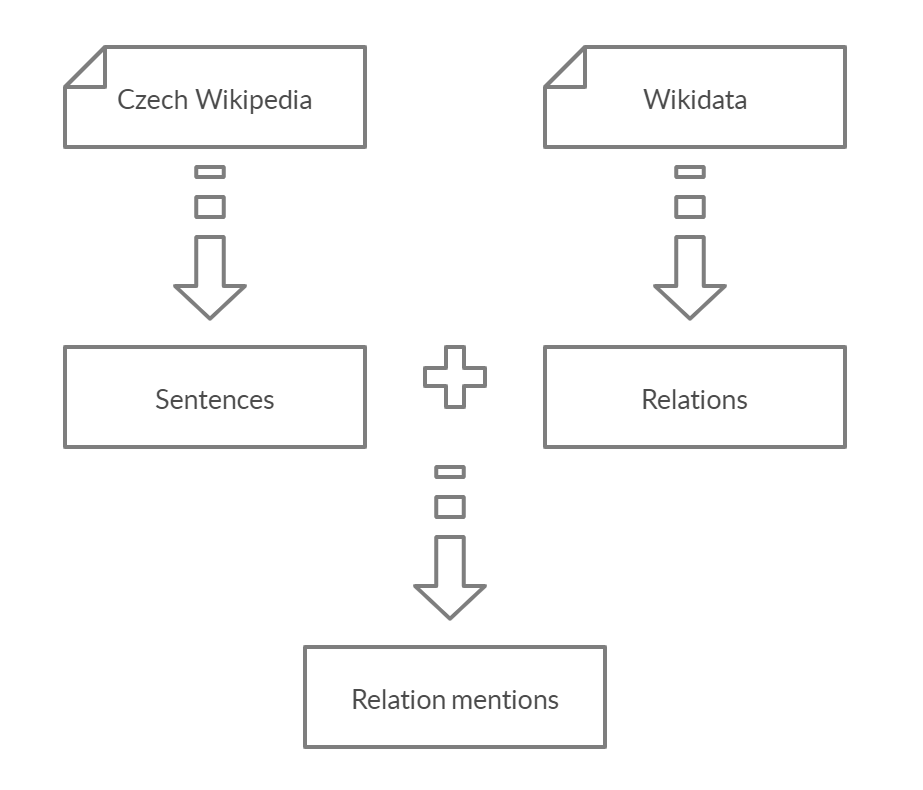
\includegraphics[width=70mm, height=60mm]{./img/a_very_simple_diagram}
\caption{A very simple diagram of dataset generation.}
\label{obr02:AVerySimple}
\end{center}
\end{figure}

Than we started the implementation and realized that this seemingly simple problem is rather complex. Even though all that we wanted was to get sentences from Wikipedia, find words or phrases, that can have relations, and link those relations from Wikidata, the number of decisions we had to make and obstacles we had to overcome was rather surprising.

As a side project, we implemented a simple viewer, that can present the dataset


\section{Data sources}

\todo{potřebujeme text + databázi a ať to jde spolu hezky propojit}

\subsection{Czech Wikipedia}

Wikipedia is a multilingual online encyclopedia created and maintained as an open collaboration project by a community of volunteers\cite{wiki:wiki} and we believe anyone reading this article is familiar with Wikipedia. From out point of view Wikipedia is a corpus of text with tagged topics of articles and some entity mentions. Czech Wikipedia contains approximately 440 000 articles and ranks top 30 across all the different language editions of Wikipedia.
\footnote{As of March 2020 according to https://en.wikipedia.org/wiki/List\_of\_Wikipedias}

A dump of Czech Wikipedia is about 1,6GB and 770MB when compressed.

\subsection{Wikidata}

Wikidata is a knowledge base, which acts as central storage of the structured data of Wikipedia and other Wikimedia projects. Just like Wikipedia, this project is freely available and edited by users (and bots). It provides the option to query the database online (for small enough queries), but it is also possible to download the database in standard formats.

The database focuses on \defineterm{items}, which represent objects, entities, concepts, etc.  The first data collected in Wikidata were links to multilingual version of Wikipedia articles on the same topic, the same Wikidata item. Each item was assigned an identifier, prefix Q and unique number, referred to as \defineterm{QID}. A label together with a description of an item should serve as a human readable identifier. Labels, descriptions a optional aliases are language dependant. 

\defineterm{Properties}, another big concept of Wikidata, can be thought of as categories of items (\wikiitem{mother}{P25} implies a category of all mothers) or as relations between items (\wikiitem{Ron Weasley}{Q173998} has a \wikiitem{mother}{P25} \wikiitem{Molly Weasley}{Q3255012}). Each property has its \defineterm{PID}, an identifier consisting of a prefix P and an unique number, and a data type for a value it can be paired with (such as an item, string, url, number or media file). \todo{hezčí formátování wikiitemm}

Information about any item is recorded in statements. Statement is a key-value pair of an property and a value of prescribed data type. For example, for \wikiitem{Ron Weasley}{Q173998} there are seven statements about his siblings:
\begin{itemize}
\item \wikiitem{sibling}{P3373} \wikiitem{Ginny Weasley}{Q187923}, 
\item \wikiitem{sibling}{P3373} \wikiitem{Fred Weasley}{Q13359612},
\item \wikiitem{sibling}{P3373} \wikiitem{George Weasley}{Q13359613} and so on
\end{itemize} . \todo{formating}

Wikidata contains over 80 000 000 items, this raises requirements on technological resources, that we will need to work efficiently with such data. Json dump of Wikidata takes 110GB of disk space or 37GB if bzip2 compressed.

\section{Used technologies}
\todo{koukli jsme se na diagram a mysleli, že celé ve spark a tak}
We chose Python to be our main programming language. To be able to work faster with bigger volume of data, we wanted to use a cluster, which leads to Spark and occasionally to some small scripts in shell/bash\todo{co je co?}. To top it, we will use MorphoDita to work with Czech language. Later, we will mention a simple Streamlit app we used to comfortably see results of our Spark queries.

In this section we will briefly introduce those technologies.
\subsection{Python}
\todo{zmiň pandy a numpy a tak}
\subsection{Spark}

\subsection{MorphoDiTa}
MorphoDiTa (Morphological Dictionary and Tagger) is an open-source tool for morphological analysis of natural language texts. It is designed to work well on inflective languages and achieves state-of-the-art results for Czech language. Internally, during training tries have been build to represent patterns for declension.  \cite{Morphodita}

\subsection{Streamlit}


\begin{figure}[p]\centering
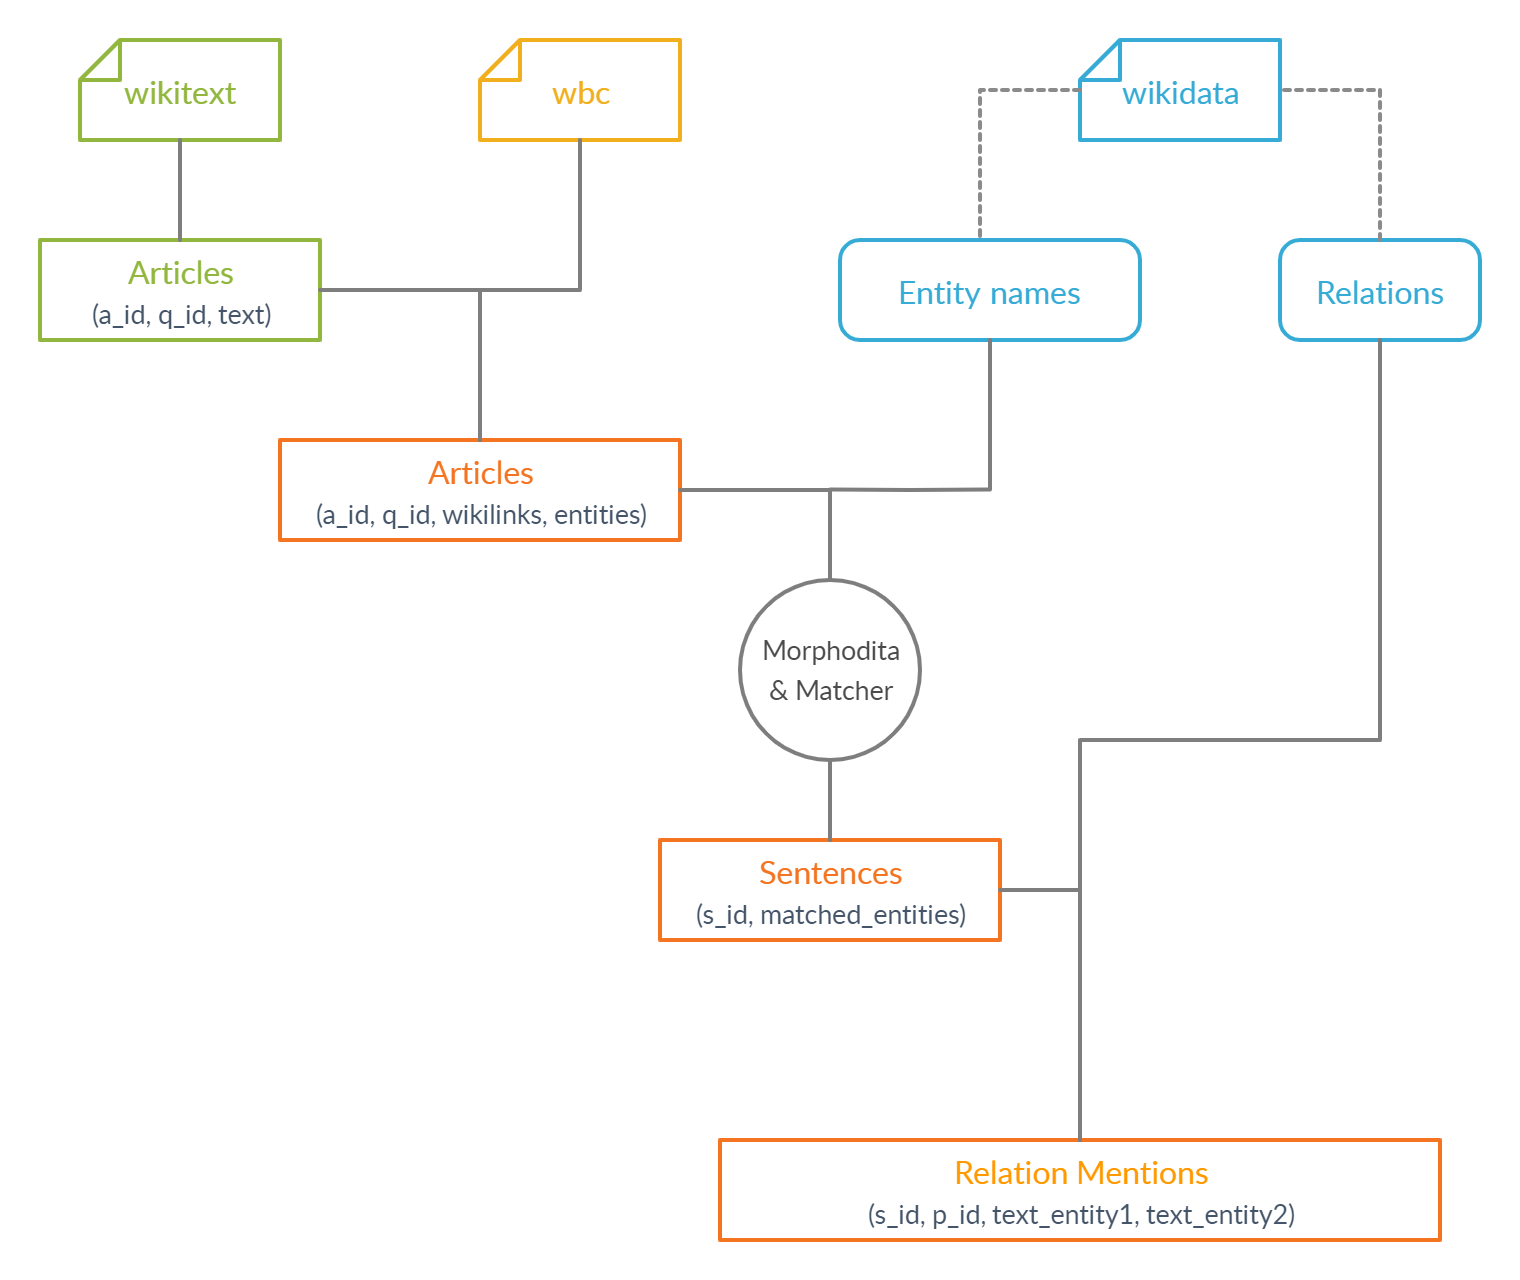
\includegraphics[width=140mm, height=117mm]{./img/Corpus_diagram}
\caption{Zjednodušený diagram výroby korpusu}
\label{obr03:Nhust}
\end{figure}


\section{Title of the second subchapter of the second chapter}
